\newpage
\section{Estudio de los modelos.}
\label{Estudio de los modelos}
\subsection{Gasolina}
\subsubsection{KYMCO Agility Carry 50 E5}
\paragraph{Descripción general}
La \textbf{\textit{KYMCO Agility Carry 50 E5}} es el mejor modelo que podemos encontrar en el mercado, según las consideraciones descritas en el \refanexo{anexo:Ciclomotor Gasolina}, para reparto, las comodidades que ofrece tanto para el usuario como para desempeñar su tarea son únicas. Orientada a obtener la máxima funcionalidad, cuenta con una parrilla en la parte delantera y otra en la trasera, útil para los repartidores, ya que soporta hasta una carga de hasta 5 \glssymbol{kg}. 

\begin{figure}[h]
    \centering
    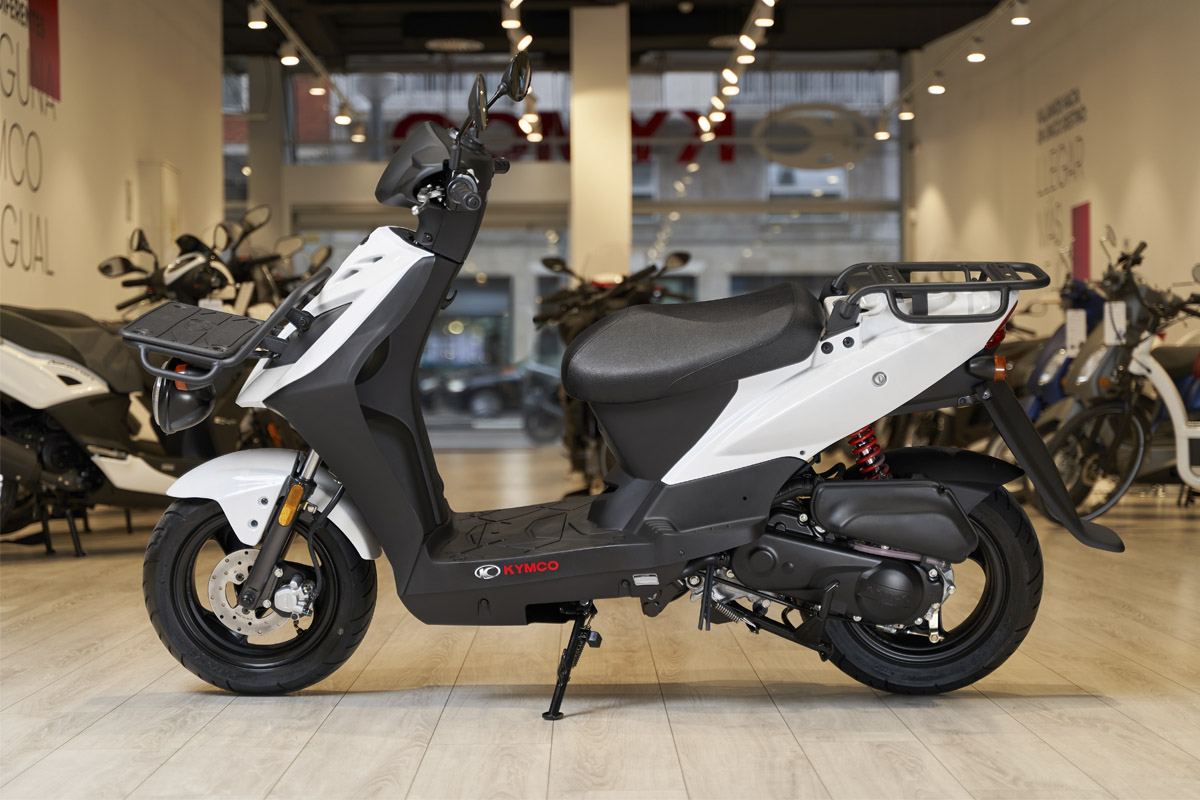
\includegraphics[scale = 0.25]{archivos/KYMCO agility carry.jpg}
    \caption{KYMCO Agility Carry 50 E5.}
    \label{fig:kymco agility carry}
\end{figure}

El motor de la \textbf{\textit{KYMCO Agility Carry 50 E5}} es de los más eficientes que hay en el mercado, se caracteriza por sus bajas emisiones y su poco consumo, tal y como se muestra en la \autoref{tab:comparacion de distintos modelos de ciclomotores de reparto}.

Además de las características que ofrece como equipo de reparto y del valor que añade a los usuarios, la empresa se ve beneficiada por su precio tan competitivo, sin lugar a dudas, su característica más destacable, ya que, por tan solo 1.999 \glssymbol{euro} la empresa puede contar con esta moto como parte de los activos. 

% \paragraph{Estudio del reparto.}
% Todos los cálculos asociados al reparto 
\paragraph{Mantenimiento y robustez}

Este modelo cuenta con un manual de usuario \cite{manualkymcociclomotor} en el que se específica el tratamiento que deben tener, los distintos elementos que componen la moto y la frecuencia con la que deben de cambiarse. 

Como se puede observar en la \autoref{fig:cambio kymco agility 50} el mantenimiento que necesita el ciclomotor no es excesivo, ya que el primer recambio de aceite es necesario después de 1000 \gls{km} o de 3 meses, lo cual nos conduce a la gran durabilidad y robustez con la que cuenta el ciclomotor.

La gran ventaja que ofrece el mantenimiento tardío radica en poder distribuirlos en el tiempo con mayor facilidad para evitar tener toda la flota en el taller y que se necesite de servicios auxiliares o de una segunda flota.

\begin{figure}[h]
    \centering
    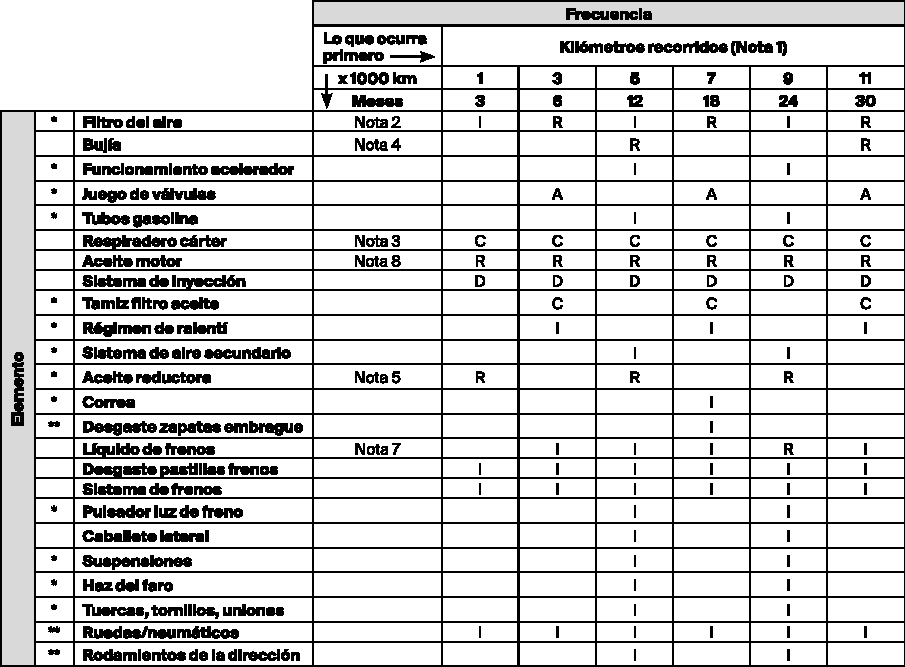
\includegraphics[scale = 1]{archivos/ManualUsuario_AgilityCity50.pdf}
    \caption{Tabla de mantenimiento del ciclomotor  KYMCO Agility Carry 50.}
    \label{fig:cambio kymco agility 50}
\end{figure}

\paragraph{Viabilidad económica}

En el \refanexo{Ciclomotor gasolina 50cc, KYMCO Agility Carry 50} se presentan una serie de cálculos relacionados con la viabilidad económica, en el que se concluye que este modelo es el más barato y el que requiere una menor inversión, cuyo dinero asciende a la cifra de 16.052,70 \glssymbol{euro} el primer año y los siguientes años 4.965,55 \glssymbol{euro}, según la \autoref{tab:Presupuesto motillo Peter}, por consiguiente esto nos da un total de 5 vehículos disponibles para el reparto, lo cual satisfará la demanda.

\paragraph{Conclusiones modelo}
Es el mejor ciclomotor con el que cuenta el mercado, está preparado para satisfacer todas las necesidades que se puedan presentar durante el desempeño de cualquier actividad de reparto, tiene un estilo moderno que combina con la imagen corporativa de cualquier empresa a una relación-calidad precio muy competitiva.
\subsubsection{KYMCO Agility Carry 125}

\paragraph{Descripción general} 
%%El ciclomotor KYMCO Aility Carry 125 es una scooter especializado para el reparto y que además cuenta con unos niveles de emisiones mínimos. Diseñado para dar una respuesta práctica ante cualquier demanda, por lo que tiene dos amplias y robustas parrillas con capacidad de 5Kg de carga para la delantera y hasta 20Kg de carga en la trasera.
Estudiando las consideraciones descritas en \refanexo{anexo_scooter_gasolina}, se ha optado de entre todos los modelos mostrados por la KYMCO Agility Carry 125 en la \autoref{fig:KYMCO Agility Carry 125}. 

\begin{figure}[h]
    \centering
    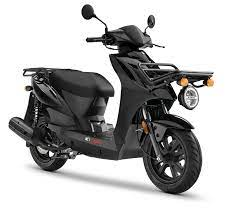
\includegraphics[scale = 0.8]{archivos/KYMCO Agility Carry 125.jpg}
    \caption{KYMCO Agility Carry 125.}
    \label{fig:KYMCO Agility Carry 125}
\end{figure}

Los motivos para elegir este modelo están basados en su especialidad para el reparto y la robustez para este tipo de tareas. La motocicleta es de una cilindrada de 125 \glssymbol{cc}, cuenta con unos niveles de emisiones mínimos y con unas parrillas delantera y trasera con capacidad de carga de hasta 5 \glssymbol{kg} y 20 \glssymbol{kg} respectivamente. Su precio actual en el mercado es de 2.149 \glssymbol{euro}.

La KYMCO Agility Carry 125 cuenta con una autonomía de 250 \glssymbol{km} debido a su depósito con capacidad de 6,5 \glssymbol{litros} y su motor de cuatro tiempos que hace que sea más eficiente. Esta autonomía es más que suficiente para realizar varias jornadas de trabajo sin repostar.

Cuenta con frenos de disco traseros y delanteros para una mayor seguridad, así como suspensiones hidráulicas para una mayor estabilidad, neumáticos de 12 pulgadas para una gran agilidad por ciudad, faros LED y un peso de tan solo 123 \glssymbol{kg}.

%El Barto

% \paragraph{Estudio del reparto.}

%  %Escoger modelo
\paragraph{Mantenimiento y robustez.}
%%Se trata de un modelo muy robusto ya que está concebido para realizar largas jornadas de trabajo.En cuanto al mantenimiento, como cualquier otra motocicleta de 125cc necesita el mantenimiento especificado en el "ANEXO X"(tabla con costes de mantenimiento).

Al ser un modelo muy robusto y concebido para realizar largas jornadas de trabajo, no tendrá tantas averías como otro modelo de motocicleta no especializada, reduciendo los costes en este aspecto.

Una motocicleta necesita mantenimiento en sus frenos, transmisión, ruedas, así como cambios de aceite y revisiones. Esto se estudia en \refanexo{anexo_precio_taller_combustible}, obteniéndose un importe anual de mantenimiento de 239 \glssymbol{euro}.
\paragraph{Viabilidad económica}
%%El coste del primer año de esta motocicleta es de 4.412,42€ y de 2.263,42€ los años sucesivos  según lo calculado en el "ANEXO X".
Para ver si es viable el gasto hay que observar el gasto fijo que supone la adquisición del equipo al completo, y posteriormente el gasto anual entre mantenimiento, seguros y combustible.

Todos los cálculos y estimaciones referentes a la viabilidad económica se pueden encontrar en la \autoref{tab:Presupuesto motocicletas de gasolina}, \refanexo{sub_anexo_calculos_motocicleta}, donde se muestran los presupuestos para ambos modelos de reparto estudiados en el estudio del reparto.

En el primer año, se han de tener en consideración el precio de mercado por unidad de las motocicletas y el número total que se van a comprar, incluyendo también el impuesto de matriculación por cada vehículo adquirido que en este modelo es de 99,77 \glssymbol{euro}. Además de esto, hay que añadir como gasto fijo inicial la adquisición del equipamiento, los cuales se enumeran en la \autoref{consideraciones_preliminares}, considerando en cada caso el número
de personal, o vehículos simultáneos en carretera.

Para los gastos anuales se debe comenzar con el coste del combustible del vehículo y el impuesto de circulación de 8,55 \glssymbol{euro}. Teniendo el precio de la gasolina, obtenido en el \refanexo{anexo_precio_taller_combustible}, se obtiene el gasto semanal y anual relacionado con el combustible. 

Los gastos relacionados con reparaciones o mantenimiento se han fijado en el \refanexo{anexo_precio_taller_combustible}, por lo que se asume un gasto mensual a cada uno.
El coste por seguro fijado es de 265 \glssymbol{euro}, lo cual se multiplicará directamente por el número de vehículos en posesión de manera mensual.

Teniendo todas las consideraciones anteriores descritas, se concluye finalmente el presupuesto necesario en el primer año y posteriores, siendo:

\begin{itemize}
    \item Presupuesto para el primer año del modelo de estudio 1 - 18.058,14 \gls{euro}
    \item Presupuesto anual del modelo de estudio 1 - 5.861,39 \gls{euro}
    \item Presupuesto para el primer año del modelo de estudio 2 - 17.591,70 \gls{euro}
    \item Presupuesto anual del modelo de estudio 2 - 5.394,95 \gls{euro}
\end{itemize}
%%Observando los resultados en \refanexo{anexo_scooter_gasolina}, \refanexo{anexo_precio_taller_combustible} y \autoref{consideraciones_preliminares_seguro} en los que se estudian detalladamente todos los costes que conlleva esta motocicleta se llega a un resultado final de que el coste que implica es de 2.149,00 \glssymbol{euro} de inversión inicial para la compra de la motocicleta y de 2.848,42\glssymbol{euro} anuales en gastos.
\paragraph{Conclusiones modelo.}
%%Es una motocicleta especializada por lo que está garantizado el perfecto cumplimiento de la tarea a realizar y una opción a considerar si no se quiere optar por los vehículos electricos.

Analizando los datos anteriores se concluye que dicha motocicleta es una opción con una gran fiabilidad, desempeño en su tarea y la opción más viable para cubrir largas distancias sin interrupción ni complicaciones. Todo esto a cambio de una mayor inversión inicial y mayor coste anual.

De las opciones que se plantean es el vehículo más seguro y que alcanza la mayor velocidad, por lo que puede realizar un mayor número de repartos, necesitando por ello menos cantidad de ellas. Dada su clasificación L3 dentro de los vehículos puede circular por autovías y autopistas en caso de que sea necesario, facilitando la labor de reparto.

Como principales inconvenientes nos encontramos con que al ser un modelo de combustión conlleva contaminación asociada, tanto medioambiental como en términos de ruido. A diferencia de las opciones eléctricas, el combustible tiene mayor coste que la energía.
\subsection{Eléctricos}
\subsubsection{Askoll eS1}
\label{apartado_moto_electrica}
\paragraph{Descripción general}
%%La motocicleta eléctrica Askoll eS1 es un scooter eléctrico de la empresa pionera en innovación de movilidad eléctrica Askoll de Italia. El scooter de la serie eS es ganador de muchos premios, incluido el Green Prix 2015.El eS1 está equipado con un motor eléctrico de 1.500 vatios con un par de 100 Nm, tiene una velocidad máxima de 45 km / h. El scooter cuenta con una batería de litio extraíble de 2,1 kWh para un alcance de 100 km y La batería se puede cargar en 6 horas.
Estudiando las consideraciones descritas en el \refanexo{anexo_scooter_electrico}, se ha escogido de entre todos los modelos mostrados el Askoll eS1 en la \autoref{fig:Askoll eS1}. 

\begin{figure}[h]
    \centering
    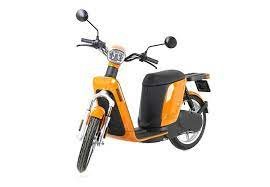
\includegraphics[scale = 0.8]{archivos/askoll es1.jpg}
    \caption{Askoll eS1.}
    \label{fig:Askoll eS1}
\end{figure}

Los motivos para elegir este modelo están basados en su gran autonomía frente a las demás opciones y un tiempo de carga bajo, lo que hace que sea la única opción realista de entre las eléctricas.

El scooter de la serie eS es ganador de muchos premios, incluido el Green Prix 2015. Está equipado con un motor eléctrico de 1.500 \glssymbol{vatios} con un par de 100 \glssymbol{par} y cuenta con una velocidad máxima de 45 \glssymbol{velocidad}. El scooter cuenta con una batería de litio extraíble de 2,1 \glssymbol{kilovatiohora} para un alcance de 100 \glssymbol{km} y la batería se puede cargar en 6 horas.

Cuenta con una autonomía de 100 \glssymbol{km} en ciudad, iluminación \gls{led}, suspensión hidráulica para una mayor estabilidad y frenos de disco para una mayor seguridad. Cuenta con neumáticos de 16 pulgadas para hacerlo más estable frente a las caídas. Un peso de tan solo 72 \glssymbol{kg} la hace muy ligera y manejable en todo tipo de situaciones.

% \paragraph{Estudio del reparto.}
%  %Escoger modelo
\paragraph{Mantenimiento y robustez}
%%Se trata de un modelo muy robusto ya que está concebido para realizar largas jornadas de trabajo. En cuanto al mantenimiento, como cualquier otra motocicleta eléctrica necesita el mantenimiento especificado en el "ANEXO X"(tabla con costes de mantenimiento).
Al ser un modelo eléctrico necesita menos mantenimiento que uno de gasolina, ya que no es necesario el cambio de aceite ni de transmisión. El modelo está construido en materiales de calidad para una mayor robustez.

Una motocicleta eléctrica necesita mantenimiento en sus frenos y ruedas, así como revisiones periódicas. Esto se estudia en el \refanexo{anexo_scooter_electrico}, obteniéndose un importe anual de mantenimiento de 126 \glssymbol{euro}.

\paragraph{Viabilidad económica}
%%El coste del primer año de esta motocicleta es de 3.348,94€ y de 663,94€ los años sucesivos  según lo calculado en el "ANEXO X".

%%Observando los resultados en \refanexo{anexo_scooter_electrico} y \autoref{consideraciones_preliminares_seguro} en los que se estudian detalladamente todos los costes que conlleva esta motocicleta se llega a un resultado final de que el coste que implica es de 2.685,00\glssymbol{euro} de inversión inicial para la compra de la motocicleta y de 753,44\glssymbol{euro} anuales en gastos.

Para ver si es factible el gasto hay que observar el gasto fijo que supone la adquisición del equipo al completo, y posteriormente el gasto anual entre mantenimiento, seguros y recargas. 

Todos los cálculos y estimaciones referentes a la viabilidad económica se pueden encontrar en la \autoref{tab:Estudio presupuestos modelo Askoll eS1}, \refanexo{sub_anexo_calculos_motocicleta_eléctrica}, donde se muestran los presupuestos para ambos modelos de reparto analizados en el estudio del reparto.

En el primer año, se han de tener en consideración el precio de mercado por unidad de las motocicletas eléctricas y el número total que se van a comprar, pues el impuesto de matriculación unitario es de 27,85 \glssymbol{euro}. Además de esto, hay que añadir como gasto fijo inicial la adquisición del equipamiento, los cuales se enumeran en la \autoref{consideraciones_preliminares}, considerando en cada caso el número de personal, o vehículos simultáneos en carretera.

Para los gastos anuales se debe comenzar con el coste de recarga del vehículo y el impuesto de circulación de 8,55 \glssymbol{euro}. Teniendo el precio de la luz, obtenido en el \refanexo{anexo_precio_taller_combustible} y el número de recargas semanales totales, junto con la capacidad de una batería, se obtiene el gasto semanal y anual relacionado con la recarga.

Los gastos relacionados con reparaciones o mantenimiento se han fijado en el \refanexo{anexo_scooter_electrico}, por lo que se asume un gasto mensual a cada uno. 

El coste por seguro fijado es de 265 \gls{euro}, lo cual se multiplicará directamente por el número de vehículos en posesión de manera mensual.

Teniendo todas las consideraciones anteriores descritas, se concluye finalmente el presupuesto necesario en el primer año y posteriores, recogidos en la \autoref{tab:Estudio presupuestos modelo Askoll eS1}, siendo:

\begin{itemize}
    \item Presupuesto para el primer año del modelo de estudio 1 - 30.475,64 \gls{euro}
    \item Presupuesto anual del modelo de estudio 1 - 5.107,09 \gls{euro}
    \item Presupuesto para el primer año del modelo de estudio 2 - 23.977,50 \gls{euro}
    \item Presupuesto anual del modelo de estudio 2 - 4.034,65 \gls{euro}
\end{itemize}

\paragraph{Conclusiones modelo.}
%%Es un modelo válido para la tarea debido a sus características y el bajo coste de mantenimiento.

Analizando los datos anteriores se concluye que dicha motocicleta es una opción con una gran autonomía, desempeño en su tarea y la opción más viable para cubrir largas distancias con pocas interrupciones. Todo esto teniendo en cuenta que tendrá que parar a recargarse cada 100 \glssymbol{km} para poder seguir con su labor de reparto.

De las opciones que se plantean es el vehículo eléctrico que alcanza la mayor velocidad y cuenta con la mayor autonomía de ellos, por lo que puede realizar un mayor número de repartos, necesitando por ello menos cantidad de ellas. Dada su clasificación dentro de los vehículos, no puede circular por autovías y autopistas en caso de que sea necesario, siendo este un factor a tener en cuenta para repartos.

Al ser un modelo de eléctrico no conlleva una contaminación, tanto medioambiental como en términos de ruido. A diferencia de las opciones de gasolina, la energía es más barata.
%\subsubsection{Bicicletas eléctricas}
%\paragraph{Descripción general}
% \paragraph{Estudio del reparto.}
%  %Escoger modelo
% \paragraph{Mantenimiento y robustez.}
% \paragraph{Viabilidad económica}
% \paragraph{Conclusiones modelo.}

\paragraph{Consideraciones previas}

Esto debe ir como ANEXO, las bicis son considerados vehículos HÍBRIDOS, no eléctricos

Las bicicletas de pedaleo deben de llevar siempre pedales y no pueden funcionar con un acelerador, por lo que es totalmente ilegal conducir por la vía pública las ``mini-bicicleta" sin pedales, según recoge el BOE y la normativa de circulación.  Según la normativa vigente, excluiremos del estudio este tipo de vehículo.

Las bicicletas eléctricas propiamente hablando son reconocidas como ``ciclo de pedaleo asistido" según el BOE N.º 124\cite{boe124}, lo que implica que aunque tienen motor eléctrico auxiliar, no pueden ser propulsadas exclusivamente haciendo uso del mismo, por lo que son vehículos híbridos entre eléctrico y manual.

\paragraph{Modelo F.Lli Schiano E-Moon}

Actualmente, una de las mejores bicicletas eléctricas del mercado calidad-precio que cumple con todas las normativas vigentes es el modelo F.Lli Schiano E-Moon, que está a la venta por 729 \glssymbol{euro}.

Respecto a sus características, posee un motor delantero ANANDA M129F de 250 \glssymbol{vatios} de potencia y 36 \glssymbol{voltios}, que permite alcanzar velocidades de hasta 25 \glssymbol{velocidad}. Presenta una batería de litio GREENWAY YJ145 36\glssymbol{voltios} 13\glssymbol{amperiohora} 468\glssymbol{vatiohora}, con una vida útil de entre 4 y 6 años y una autonomía de hasta 120 \glssymbol{km} con 6 horas de carga completa. 

Su sistema de frenado es V-Brake en las ruedas delantera y trasera, ambos neumáticos son Kenda de 26 pulgadas. El cuerpo de la bicicleta no es plegable, es de una aleación de aluminio resistente, aunque no ligera (25 \glssymbol{km}). Consta de una caja de cambios Shimano Tourney TY21 de 7 velocidades, un timbre, una luz delantera y otra trasera. 
Cumple todos los requisitos para ser considerada una bicicleta eléctrica:

\begin{itemize}
\item Tener dos ruedas, tal como considera El Real Decreto 2822/1998, de 23 de diciembre, que aprueba el Reglamento General de Vehículos.\cite{boe2822}
\item Contar con un motor eléctrico cuya potencia máxima no exceda los 250 \glssymbol{vatios}.
\item Alcanzar una velocidad máxima asistida de 25 \glssymbol{velocidad}.
\item El motor ha de encender con el pedaleo y apagarse al llegar a 25 \glssymbol{velocidad} o cuando el pedaleo cese.
\end{itemize}

Al cumplir todos los requisitos anteriores no es necesario seguro obligatorio, matrícula, tarjeta de inspección técnica, casco ni permiso de conducción para circular por las vías públicas. No obstante, sí es necesario que el vehículo cuente con:


\begin{itemize}
\item Doble sistema de frenado, un freno para la rueda delantera y otro para la trasera.
\item Timbre. 
\item Luces de posición. La luz delantera debe ser de color blanco y la posterior de color rojo.
\item Señalización trasera.
\end{itemize}

Todas las especificaciones numeradas están incluidas en el modelo seleccionado.

Las bicicletas eléctricas no tienen restricciones relevantes de circulación en la vía pública, pueden usar los carriles bici o la carretera en su defecto. Además, si fuese necesario pueden circular por el arcén en autovías.

\paragraph{Viabilidad del modelo}

Tal como se recoge en el plano 3 del Anexo “X”, el rango de alcance de los repartos es de 6 \glssymbol{km} poniendo como centro la localización de la sede.

Haciendo uso de los cálculos recogidos en el anexo “X” son necesarias unas 8 bicicletas eléctricas, las cuales se usarán durante todo el día y se recargarán por la noche, en el horario de cierre del negocio (24:00-9:00).

Suponiendo una revisión mensual de mantenimiento, el precio de la luz en el horario en el que se producirá la recarga de los vehículos, el coste de adquisición de los vehículos recogidos en la tabla "x". 

El coste de adquisición de los vehículos, junto y el resto de servicios requeridos por los mismos, supondría \glssymbol{euro}, tal como se expresa en la ecuación "x"

En los años siguientes, el coste en vehículos sería de aproximadamente ...\glssymbol{euro}.

De este modo, se estima que en 10 años la empresa habrá invertido ... \glssymbol{euro} en los vehículos, incluido mantenimiento, reparaciones y recargas.

La empresa ha de invertir un coste de ... bastante primer año de adquisición de los vehículos es de …. € y él anualmente se gastarían … \glssymbol{euro}.


SUPUESTA TABLA:

Precio estimado de la luz en el tramo horario 24:00-6:00 con base en los datos de los últimos meses en ese tramo horario: 0.2645 \glssymbol{euro}/\glssymbol{kilovatiohora}

Precio mantenimiento general bicicleta eléctrica en Feuvert:44,95 \glssymbol{euro}/anuales



En vista de los resultados económicos y de buena imagen de la empresa hacia el consumidor debido al método de reparto ecológico, es evidente que es una buena opción a tener en cuenta entre los distintos vehículos del mercado. No obstante, ha de considerarse que para ciertos trayectos próximos a los 6 km o que impliquen el uso de algún tramo de autovía, no es aconsejable el uso de este modelo eléctrico por seguridad del transportista y/o por exceso del tiempo de reparto deseado. Asimismo, las opciones de estacionamiento de bicicletas son limitadas, semáforos, farolas y barandillas no están permitidas, por lo que se ha de localizar un parking de bicicletas o estacionarlas del mismo modo que una moto convencional (en este último método, sería necesario también el uso de una cadena especial).

MIS fuentes:
https://www.feuvert.es/movilidad-bicis-mantenimiento/r132.html
https://tarifaluzhora.es/
https://www.almaskater.com/bicicletas-electricas-baratas/
https://www.boe.es/boe/dias/2014/05/22/pdfs/BOE-A-2014-5399.pdf

\subsubsection{Infiniton CITYJam Pro}
\label{apartado_patinetes}
\paragraph{Descripción general}

Estudiando las consideraciones descritas en el \refanexo{anexo_patienete eléctrico}, se ha optado de entre todos los modelos por la Infiniton CITYJam Pro \cite{infinitoncityjam}, mostrado en la \autoref{fig:Infinity CityJam}.

\begin{figure}[h]
    \centering
    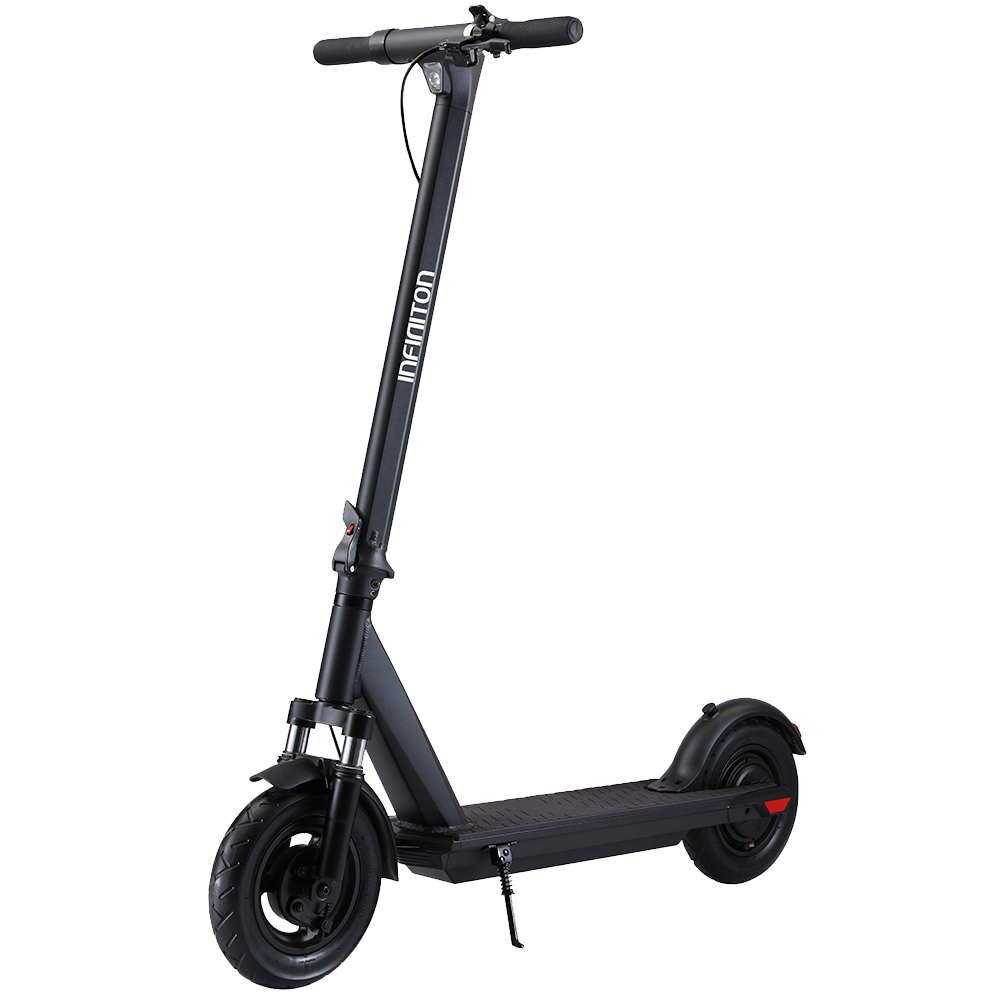
\includegraphics[scale = 0.2]{archivos/cityjam-pro-negro.jpg}
    \caption{Infiniton CITYJam Pro.}
    \label{fig:Infinity CityJam}
\end{figure}

Los motivos para elegir este modelo se fundamentan en su larga autonomía frente a los demás, y su capacidad en batería, permitiendo cargas más económicas y espaciadas en el tiempo. No se han tenido en consideración la inclinación del terreno o el peso máximo, dado que el rango de destino, terreno de la ciudad, y tipos de pedidos no suponen la  importancia necesaria.

La Infiniton CITYJam Pro tiene una autonomía de entre 40-45 \glssymbol{km} de distancia gracias a su batería de 350 \glssymbol{vatiohora}. Al igual que otros modelos en el mercado, cuenta con un sistema de recarga de energía cuando se frena, permitiendo prolongar la vida de cada carga.

Dispone de mucha estabilidad y durabilidad gracias al uso de acero resistente en su fabricación, junto con tres sistemas de frenos distintos y luces frontales y traseras para garantizar la seguridad del usuario.

La potencia que ofrece este modelo permite transportar cargas de hasta 100 \glssymbol{kg}, siendo suficiente para transportar al repartidor junto con el pedido.

\paragraph{Mantenimiento y robustez}

El patinete está fabricado con los materiales necesarios para soportar el día a día frente a un uso de ciudad. Además de ello, cuenta con un grado de protección IP54, controlado por la norma internacional CEI 60529 \cite{une60529}, capaz de soportar lluvia y polvo sin ningún tipo de problema.

El mantenimiento \cite{mantenimientopatinete} es más sencillo y económico comparado con un coche o una moto. Se recomienda emplear siempre piezas originales y no utilizar cargadores distintos al original. La limpieza del vehículo se puede realizar con ayuda de un trapo y cepillo, evitando el uso de mangueras de presión localizados en lavaderos de coches. 

Por otro lado, el modelo que estudiamos tiene ruedas de diez pulgadas, por lo que su durabilidad frente al desgaste va a ser alta. En caso de daño o fin de su vida útil, se pueden sustituir manualmente con recambios, sin necesidad de acudir a un taller especializado.

En referencia al sistema electrónico o la batería, se ha de evitar manipularlo, y en caso de avería llevarlo a un taller especializado. Las reparaciones dependen del daño y del taller al que se acuda, pero su precio no excede el de una avería de moto u otros tipos de vehículos.

Además de todo lo anterior, tal y como se indica en el \refanexo{anexo_precio_taller_combustible}, se incluye una cantidad fija de ahorro para caso de siniestro y sustitución de patinete.

\paragraph{Viabilidad económica}

Para ver si es aceptable el gasto hay que observar el gasto fijo que supone la adquisición del equipo al completo, y posteriormente el gasto anual entre mantenimiento, seguros y recargas. 

Todos los cálculos y estimaciones referentes a la viabilidad económica se pueden encontrar en la \autoref{tab: analisis_presupuestos_patienetes}, \refanexo{sub_anexo_calculos_patinete}, donde se muestran los presupuestos para ambos modelos de reparto estudiados en el estudio del reparto.

En el primer año, se han de tener en consideración el precio de mercado por unidad de los patinetes y el número total de patinetes que se van a comprar, según el \refanexo{anexo_calculos_sobre_vehiculos} son necesarios un total de 20 patinetes según la hipótesis de reparto de 5 \glssymbol{km} y 16 según la hipótesis de pedidos dobles. Además de esto, hay que añadir como gasto fijo inicial la adquisición del equipamiento, los cuales se enumeran en la \autoref{consideraciones_preliminares}, considerando en cada caso el número de empleados, o vehículos simultáneos en carretera que en este modelo serán 8 y 7, respectivamente.

Para los gastos anuales se debe comenzar con el coste de recarga del vehículo. Teniendo el precio de la luz, obtenido en el \refanexo{anexo_precio_taller_combustible} y el número de recargas semanales totales, junto con la capacidad de una batería, se obtiene el gasto semanal y anual relacionado con la recarga.

Los gastos relacionados con reparaciones o mantenimiento se han fijado en el \refanexo{anexo_precio_taller_combustible}, por lo que se asume un gasto mensual a cada uno. 

El coste por seguro fijado es de 35 \gls{euro}, lo cual se multiplicará directamente por el número de vehículos en posesión de manera mensual.

Teniendo todas las consideraciones anteriores descritas, se concluye finalmente el presupuesto necesario en el primer año y posteriores, siendo:

\begin{itemize}
    \item Presupuesto para el primer año del modelo de estudio 1 - 12.323,53 \gls{euro}
    \item Presupuesto anual del modelo de estudio 1 - 3.873,05 \gls{euro}
    \item Presupuesto para el primer año del modelo de estudio 2 - 9.926,05 \gls{euro}
    \item Presupuesto anual del modelo de estudio 2 - 3.096,81 \gls{euro}
\end{itemize}


\paragraph{Conclusiones modelo.}

Analizando los datos obtenidos, se llega a la conclusión que en cuestiones económicas, el patinete eléctrico es una de las opciones más baratas del mercado. A pesar de ser necesario una flota grande inicial para disponer siempre de un vehículo operativo, el coste sigue siendo menor que otras alternativas.

El coste energético es proporcional al precio de la electricidad, aunque comparado con la gasolina sigue siendo una alternativa eficiente y económica.

Los inconvenientes de este modelo de transporte son por un lado la seguridad del conductor, debido a lo vulnerable que es a los accidentes en carretera y condiciones meteorológicas, y por otro lado la cantidad necesaria de vehículos para garantizar el correcto funcionamiento del servicio, debido a que implica la posesión de las tomas de corriente suficientes para realizar múltiples cargas simultaneas.
\subsection{Comparativa entre los modelos estudiados}
A modo de resumen, la \autoref{tab:resumen_final}
incluye el número de vehículos necesarios para cada una de las opciones estudiadas a lo largo de esta sección, junto con sus precios actuales en el mercado, que definirá en gran medida la inversión inicial. Asimismo, se recogen el número de vehículos que han de estar simultáneamente en carretera, lo cual delimita la cantidad de recurso humano que debe invertir la empresa dependiendo del modelo elegido.

% Tabla
\begin{table}[H]
\centering
\begin{tabular}{l|c|c|c|c|}
\cline{2-5}
 & \multicolumn{1}{l|}{Ciclomotor} & \multicolumn{1}{l|}{Motocicleta} & \multicolumn{1}{l|}{Patinete eléctrico} & \multicolumn{1}{l|}{Motocicleta eléctrica} \\ \hline
\multicolumn{1}{|l|}{Coste  unitario vehículo (\glssymbol{euro})} & 1.999,00 & 2.149,00 & 376,62 & 2.685,00 \\ \hline
\multicolumn{1}{|l|}{\begin{tabular}[c]{@{}l@{}}N º vehículos totales \\ necesarios caso 1\end{tabular}} & 5 & 5 & 20 & 9 \\ \hline
\multicolumn{1}{|l|}{\begin{tabular}[c]{@{}l@{}}N º vehículos totales \\ necesarios caso 2\end{tabular}} & 5 & 5 & 16 & 7 \\ \hline
\multicolumn{1}{|l|}{\begin{tabular}[c]{@{}l@{}}N º vehículos simultáneos \\ en carretera, caso 1\end{tabular}} & 5 & 5 & 8 & 5 \\ \hline
\multicolumn{1}{|l|}{\begin{tabular}[c]{@{}l@{}}N º vehículos simultáneos\\  en carretera, caso 2\end{tabular}} & 5 & 5 & 7 & 5 \\ \hline
\end{tabular}
\caption{Resumen número de vehículo imprescindibles según cada modelos estudiados}
\label{tab:resumen_final}
\end{table}
Una vez analizados diversos vehículos factibles para el reparto de comida a domicilio, se han realizado también la \autoref{fig:comparativa_caso_1} donde se comparan los costes económicos de las opciones estudiadas para el supuesto de que cada reparto incluya un único pedido y la \autoref{fig:comparativa_caso_2}, referente a la hipótesis de los pedidos dobles.

\begin{figure}[h]
    \centering
    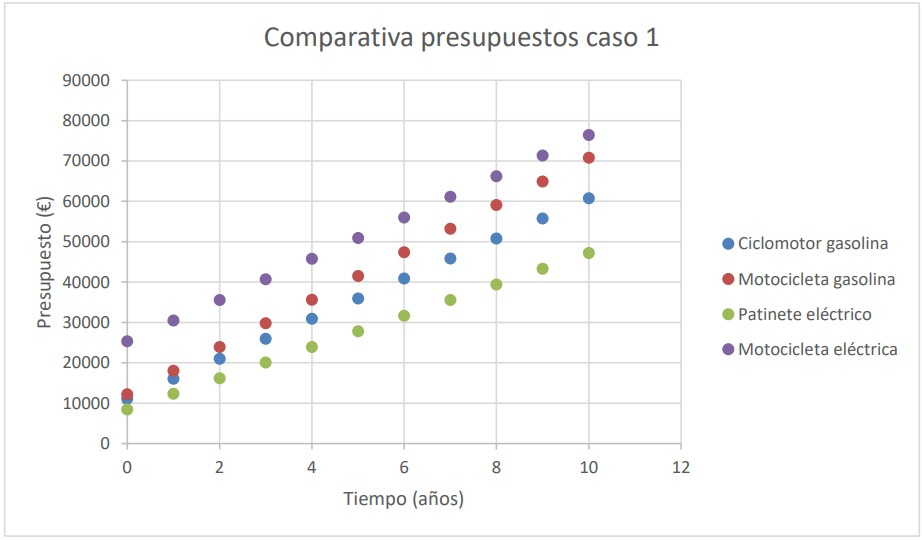
\includegraphics[scale = 0.4]{archivos/Comparativa_presupuestos_caso_1.jpeg}
    \caption{Comparación de presupuestos de los vehículos para repartos individuales}
    \label{fig:comparativa_caso_1}
\end{figure}

\begin{figure}[h]
    \centering
    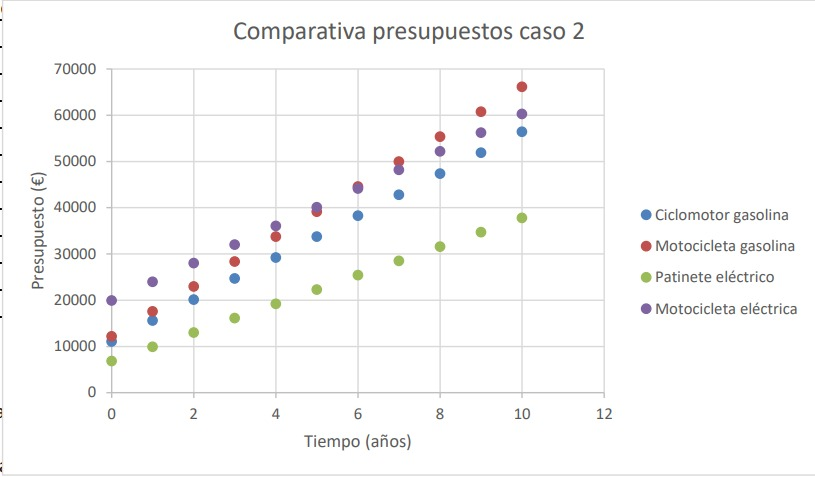
\includegraphics[scale = 0.4]{archivos/Comparativa_presupuestos_caso_2.jpeg}
    \caption{Comparación de presupuestos de los vehículos para repartos dobles}
    \label{fig:comparativa_caso_2}
\end{figure}

Se observa que la \autoref{fig:comparativa_caso_1}, las motocicletas eléctricas, destacan como vehículo más caro, aunque ciertamente, la recta que define sus presupuestos tiende a aplanarse y abaratarse en un periodo de tiempo mayor. No obstante, si se observa la \autoref{fig:comparativa_caso_2}, apenas hay diferencia de precio entre la motocicleta eléctrica y las de gasolina.



Económicamente, la opción más rentable son los patinetes eléctricos en ambas figuras y la peor opción es la motocicleta de gasolina, seguida de la motocicleta eléctrica. No obstante, partiendo de la premisa inicial de cubrir un radio de 6 \glssymbol{km} desde el establecimiento que impone la empresa \textit{DELICIOUS BURGER S.A.}; es evidente que el uso de patines eléctricos para entregar pedidos a 5 o 6 km de distancia no es lo ideal, además de tener que atravesar un tramo de autovía (prohibido por ley para este tipo de vehículos), el cliente recibiría su pedido con retardo y frío. Por consiguiente, se ha decidido indagar una alternativa a usar un único vehículo.

\subsection{Opción óptima}
\subsubsection{Justificación de la elección}

En el \refanexo{anexo_scooter_electrico} y en el \refanexo{anexo_patienete eléctrico} se ha debatido la mejor opción dentro de la gama de motocicletas eléctricas y patinetes eléctricos, respectivamente. En consecuencia, se plantea una alternativa eficiente y coherente que cohesiona a la perfección la autonomía que proporciona el modelo de motocicleta Askoll eS1, con el precio competitivo de los patinetes Infiniton CITYJam Pro, cuyas características se encuentran detalladas en la
\autoref{apartado_moto_electrica} y en la \autoref{apartado_patinetes} de esta \autoref{Estudio de los modelos}.


Tomando en consideración que el reparto de los pedidos es homogéneo en todas las franjas horarias, el radio de alcance máximo es de 6 \glssymbol{km} que aparece en el \hyperref[plano:radio]{\hyperlink{plano:radio}{Plano 3}} del \refanexo{anexo_planos}, y la longitud de los pedidos contando ida y vuelta de media oscila entre los 5 y los 7,5 \glssymbol{km}; se puede suponer que la longitud de los recorridos también posee cierta uniformidad. Por ello, se estima que el número de pedidos que se han de repartir en un radio de 4 a 6 \glssymbol{km} desde el establecimiento, supondrá a lo sumo un 33 \% de los mismos.

La solución que se plantea es que las motocicletas eléctricas cubran ese porcentaje de pedidos lejanos en todos y cada uno de los tramos horarios estudiados, mientras que los pedidos de corto alcance se realicen en patinetes. De este modo, se elimina el problema que presentan los patinetes al no poder alcanzar todas las áreas donde se debían realizar las entregas, al mismo tiempo que se mejora el tiempo de entrega en pedidos cortos porque los patinetes no necesitan ser estacionados, pueden acompañar a su conductor hasta la misma puerta del cliente.

\subsubsection{Estudio del reparto}
Una motocicleta eléctrica del modelo Askoll eS1 es capaz de realizar unos 100 \glssymbol{km} a carga completa, lo que equivale a 20 pedidos, suponiendo que los repartos tienen una duración media de 5 \glssymbol{km}, o 13 pedidos si se suponen 7,5 \glssymbol{km}. Realizando los mismos cálculos que en el \autoref{anexo_calculos_sobre_vehiculos}, pero reduciendo el número de pedidos a realizar en cada tramo horario, se obtiene que son necesarias aparentemente unos 18 patinetes para la primera hipótesis contemplada (repartos individuales de 5 km) y 16 patinetes para el caso de realizar repartos dobles de 7,5 \glssymbol{km} de ida y vuelta, según la \autoref{tab: analisis_detallado_patinete_5km_22} y la \autoref{tab: analisis_detallado_patinete_7,5km_22}.

\begin{table}[H]
\centering
\begin{tabular}{l|c|c|c|c|}
\cline{2-5}
 & \begin{tabular}[c]{@{}c@{}}TRAMO \\ HORARIO 1\end{tabular} & \begin{tabular}[c]{@{}c@{}}TRAMO \\ HORARIO 2\end{tabular} & \begin{tabular}[c]{@{}c@{}}TRAMO \\ HORARIO 3\end{tabular} & \begin{tabular}[c]{@{}c@{}}TRAMO \\ HORARIO 4\end{tabular} \\ \cline{2-5} 
 & \begin{tabular}[c]{@{}c@{}}Lunes-Jueves \\ (9:00-20:00)\end{tabular} & \begin{tabular}[c]{@{}c@{}}Lunes-Jueves \\ (20:00-0:00)\end{tabular} & \begin{tabular}[c]{@{}c@{}}Viernes-Domingo \\ (9:00-20:00)\end{tabular} & \begin{tabular}[c]{@{}c@{}}Viernes-Domingo \\ (20:00-1:00)\end{tabular} \\ \hline
\multicolumn{1}{|l|}{Nº pedidos} & 30 & 40 & 44 & 90 \\ \hline
\multicolumn{1}{|l|}{\begin{tabular}[c]{@{}l@{}}Distancia total a \\ recorrer \glssymbol{km}\end{tabular}} & 150 & 200 & 220 & 450 \\ \hline
\multicolumn{1}{|l|}{\begin{tabular}[c]{@{}l@{}}Tiempo total de \\ reparto \glssymbol{minuto} \end{tabular}} & 660 & 240 & 660 & 300 \\ \hline
\multicolumn{1}{|l|}{\begin{tabular}[c]{@{}l@{}}Tiempo estimado \\ por pedido (\glssymbol{minuto}/pedido)\end{tabular}} & 20 & 20 & 20 & 20 \\ \hline
\multicolumn{1}{|l|}{\begin{tabular}[c]{@{}l@{}}Nº pedidos realizables \\ por vehículo\end{tabular}} & 33 & 12 & 33 & 15 \\ \hline
\multicolumn{1}{|l|}{\begin{tabular}[c]{@{}l@{}}Nº vehículos simultáneos \\ necesarios\end{tabular}} & 1 & 4 & 2 & 6 \\ \hline
\multicolumn{1}{|l|}{Nº de turnos de vehículos} & 4 & 8 & 3 & 2 \\ \hline
\multicolumn{1}{|l|}{\begin{tabular}[c]{@{}l@{}}Nº vehículos totales \\ necesarios\end{tabular}} & 4 & 8 & 6 & 12 \\ \hline
\end{tabular}
\caption{Análisis detallado del reparto en patinete con viajes de 5 \glssymbol{km}.}
\label{tab: analisis_detallado_patinete_5km_22}
\end{table}



\begin{table}[H]
\centering
\begin{tabular}{l|c|c|c|c|}
\cline{2-5}
 & \begin{tabular}[c]{@{}c@{}}TRAMO \\ HORARIO 1\end{tabular} & \begin{tabular}[c]{@{}c@{}}TRAMO \\ HORARIO 2\end{tabular} & \begin{tabular}[c]{@{}c@{}}TRAMO \\ HORARIO 3\end{tabular} & \begin{tabular}[c]{@{}c@{}}TRAMO \\ HORARIO 4\end{tabular} \\ \cline{2-5} 
 & \begin{tabular}[c]{@{}c@{}}Lunes-Jueves \\ (9:00-20:00)\end{tabular} & \begin{tabular}[c]{@{}c@{}}Lunes-Jueves \\ (20:00-0:00)\end{tabular} & \begin{tabular}[c]{@{}c@{}}Viernes-Domingo \\ (9:00-20:00)\end{tabular} & \begin{tabular}[c]{@{}c@{}}Viernes-Domingo \\ (20:00-1:00)\end{tabular} \\ \hline
\multicolumn{1}{|l|}{Nº pedidos dobles} & 7 & 12 & 17 & 47 \\ \hline
\multicolumn{1}{|l|}{\begin{tabular}[c]{@{}l@{}}Distancia total a \\ recorrer (\glssymbol{km})\end{tabular}} & 52,5 & 90 & 127,5 & 352,5 \\ \hline
\multicolumn{1}{|l|}{\begin{tabular}[c]{@{}l@{}}Tiempo total de \\ reparto doble (\glssymbol{minuto})\end{tabular}} & 660 & 240 & 660 & 300 \\ \hline
\multicolumn{1}{|l|}{\begin{tabular}[c]{@{}l@{}}Tiempo estimado por \\ pedido doble (\glssymbol{minuto}/pedido)\end{tabular}} & 32,5 & 32,5 & 32,5 & 32,5 \\ \hline
\multicolumn{1}{|l|}{\begin{tabular}[c]{@{}l@{}}Nº pedidos dobles \\ realizables por vehículo\end{tabular}} & 20 & 7 & 20 & 9 \\ \hline
\multicolumn{1}{|l|}{\begin{tabular}[c]{@{}l@{}}Nº vehículos simultáneos \\ necesarios\end{tabular}} & 1 & 2 & 1 & 6 \\ \hline
\multicolumn{1}{|l|}{Nº de turnos de vehículos} & 2 & 2 & 4 & 2 \\ \hline
\multicolumn{1}{|l|}{\begin{tabular}[c]{@{}l@{}}Nº vehículos totales \\ necesarios\end{tabular}} & 2 & 4 & 4 & 12 \\ \hline
\end{tabular}
\caption{Análisis detallado del reparto en patinete con viajes de 7,5 \glssymbol{km}.}
\label{tab: analisis_detallado_patinete_7,5km_22}
\end{table}

Seguidamente, se analizan mediante gráficas el número de patinetes necesarios para las franjas horarias donde se produce el \gls{cuello de botella}, es decir, los fines de semana. Todo esto dependerá sustancialmente del tiempo que dura la recarga de los patinetes.

En la \autoref{fig:patinetes_caso1_2} aparecen representados en azul los 3 turnos de 2 patinetes vehículos cada uno, así como los 2 turnos de 6 patinetes por la tarde (color verde). Según el tiempo de recarga de las baterías, los dos patinetes del primer turno de la mañana se pueden emplear en el segundo turno de vehículos de la tarde. En consecuencia, para el primer caso estudiado solo son necesarios 16 patinetes en total.

\begin{figure}[H]
    \centering
    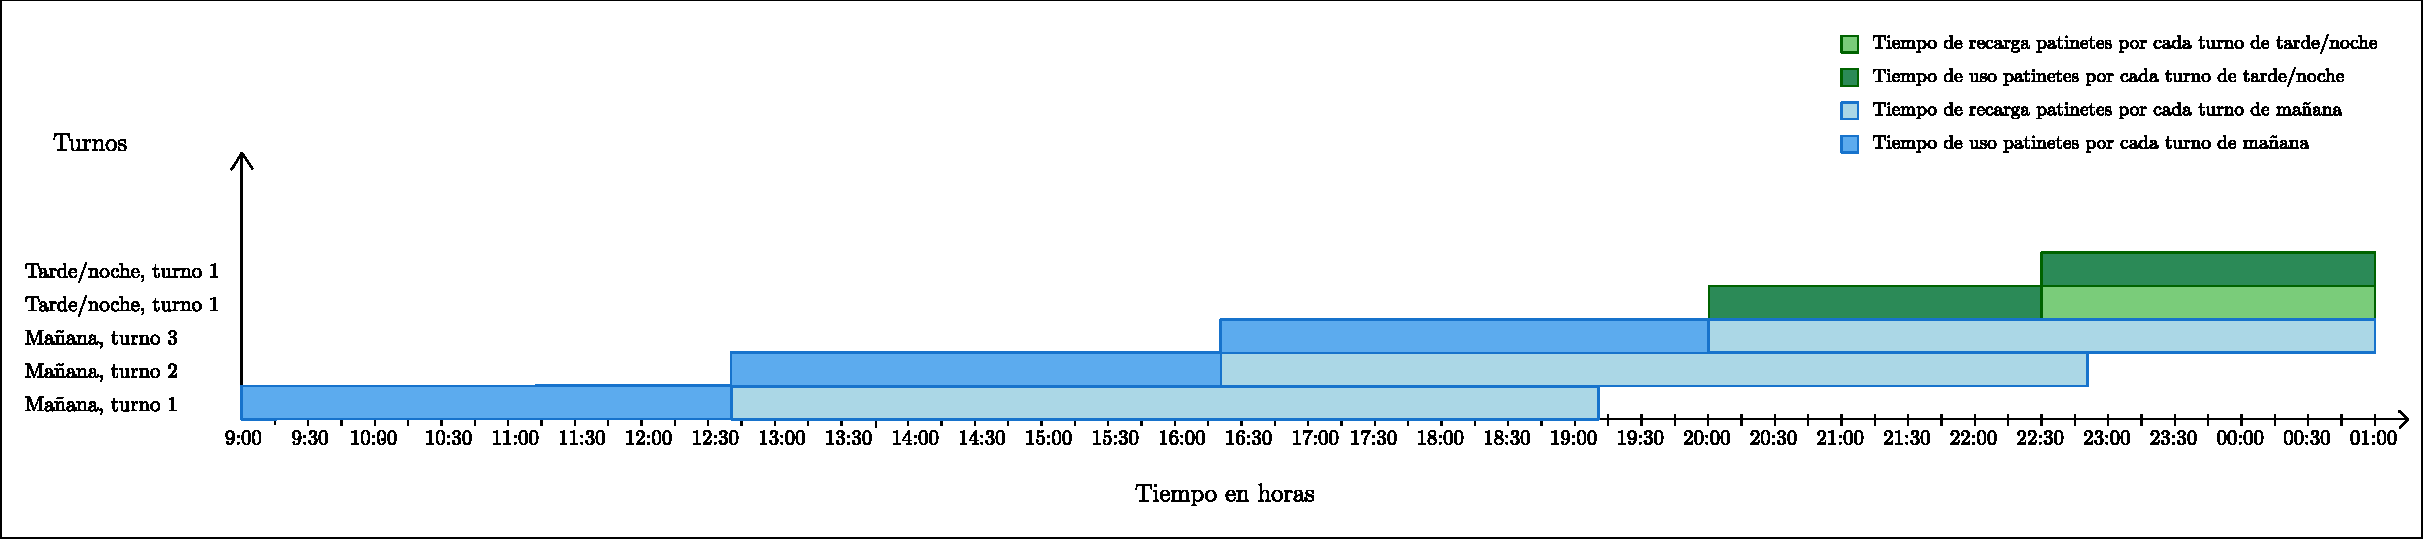
\includegraphics[width= \textwidth, height=12em]{archivos/caso2_patinetes.pdf}
    \caption{Representación turnos minorados de patinetes en viajes de 5 \glssymbol{km}.}
    \label{fig:patinetes_caso1_2}
\end{figure}

Igualmente, en la \autoref{fig:patinetes_caso2_2} se observa que 2 de los patinetes del turno de mañana se pueden recargar y utilizar en el horario posterior, por lo que para esa hipótesis solo son necesarios 14 patinetes.

\begin{figure}[H]
    \centering
    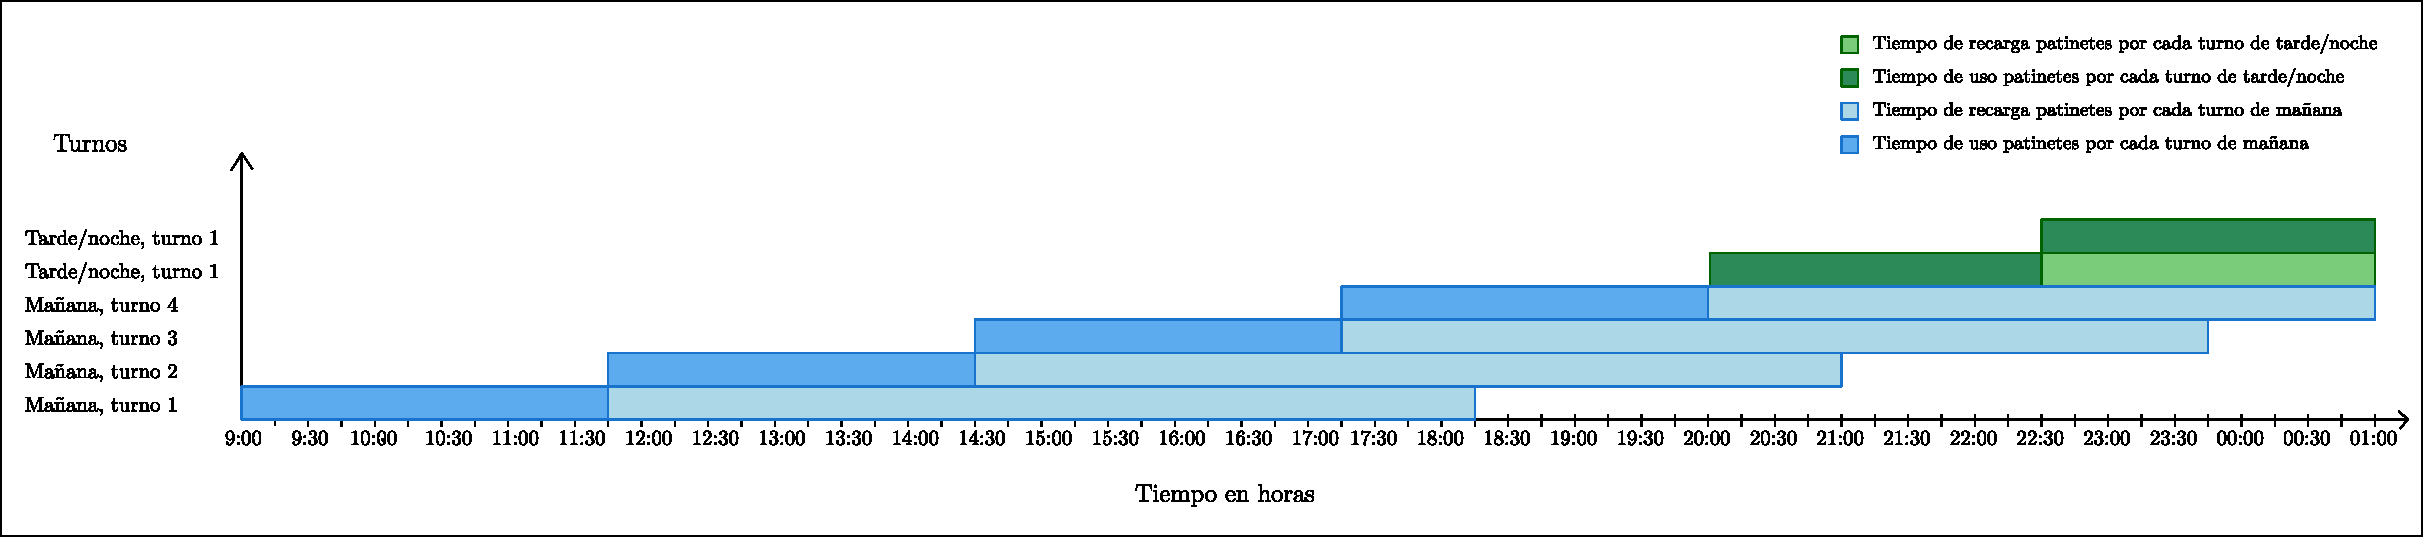
\includegraphics[width= \textwidth, height=12em]{archivos/caso1_patinetes.pdf}
    \caption{Representación turnos minorados de patinetes en viajes de 7,5 \glssymbol{km}.}
    \label{fig:patinetes_caso2_2}
\end{figure}

\subsubsection{Presupuestos}
Finalmente, para hallar el presupuesto de esta opción híbrida se deben tener en cuenta diversos factores. 

Como se ha mencionado anteriormente, se supone  que las motocicletas cubren el 33\% de los repartos, por ello los días entre semana se empleará una motocicleta para todo el día, mientras que en los fines de semana se usará una motocicleta en el turno de mañana y en el turno de tarde se ha de emplear la motocicleta del turno anterior además de otra a plena carga.

Respecto a los cálculos se ha de sumar el número de patinetes y sus costes asociados, así como los dos patinetes y sus respectivos costes, todo queda recogido en la \autoref{tab: analisis_presupuestos_patinetes_y_motos}. En estos cálculos se han empleado datos de la \autoref{tabla:tabla_datos_comunes}, de la \autoref{tab: analisis_presupuestos_patienetes} y de la \autoref{tab:Estudio presupuestos modelo Askoll eS1} debido a que estos modelos ya se han analizado en detalle en el \autoref{anexo_calculos_sobre_vehiculos}.

\begin{table}[H]
\centering
\begin{tabular}{|l|c|}
\hline
Nº patinetes necesarios caso 1 & 16 \\ \hline
Nº patinetes necesarios caso 2 & 14 \\ \hline
Nº motocicletas necesarias en ambos casos & 2 \\ \hline
Nº recargas semanales patinetes caso 1 & 102 \\ \hline
Nº recargas semanales patinetes caso 2 & 72 \\ \hline
Nº recargas semanales motocicletas caso 1 & 10 \\ \hline
Nº recargas semanales motocicletas caso 2 & 10 \\ \hline
Presupuesto anual en recargas caso 1 (\glssymbol{euro}) & 330,01 \\ \hline
Presupuesto anual en recargas caso 2 (\glssymbol{euro}) & 268,90 \\ \hline
Presupuesto para vehículos primer año caso 1 (\glssymbol{euro}) & 16.536,67 \\ \hline
Presupuesto para vehículos primer año   caso 2 (\glssymbol{euro}) & 15.362,72 \\ \hline
Presupuesto para vehículos anual  caso 1 (\glssymbol{euro}) & 4.205,91 \\ \hline
Presupuesto para vehículos anual caso 2 (\glssymbol{euro}) & 3.785,20 \\ \hline
Presupuesto en vehículos a 10 años, caso 1 (\glssymbol{euro}) & 54.389,9 \\ \hline
Presupuesto en vehículos a 10 años, caso 2 (\glssymbol{euro}) & 49.429,53 \\ \hline
\end{tabular}
\caption{Análisis de los presupuestos opción óptima.}
\label{tab: analisis_presupuestos_patinetes_y_motos}
\end{table}


% 3.4.4. Ventajas y desventajas
Las ventajas que proporciona este modelo híbrido de reparto usando 2 vehículos 100\% son diversas. Cabe destacar que los patinetes eléctricos en repartos de corto alcance agilizan la entrega de pedidos y minimizan el riesgo de robos de vehículos fuera del local porque pueden acompañar en todo momento al conductor. Además, económicamente este vehículo es el más barato.

Del mismo modo, las motocicletas eléctricas proporcionan gran independencia, los repartos de larga distancia quedan cubiertos en el tiempos estimado sin restricciones de circulación. Al contrario de lo que ocurre con los patinetes, las motocicletas pueden realizar recorridos más largos y atravesar tramos de carretera, como el necesario para alcanzar el área próxima a Churriana

Respecto a las desventajas, solo hay que incidir en el hecho de que al usar motocicletas eléctricas, el presupuesto se eleva y al usar patinetes eléctricos, se requieren más empleados como repartidores que usando otro tipo de vehículos.

De acuerdo con lo expuesto en este subapartado, junto con la buena imagen que aportan los vehículos eléctricos frente a los de gasolina a la empresa, el uso de vehículos 100\% eléctricos como son el modelo Askoll eS1 y el Infiniton CITYJam Pro es la opción más apropiada.
